%%%%%%%%%%%%%%%%%%%%%%%%%%%%%%%%%%%%%%%%%%%%%%%%%%%%%%%%%%%%%%%%%
% MUW Presentation
% LaTeX Template
% Version 1.0 (27/12/2016)
%
% License:
% CC BY-NC-SA 4.0 (http://creativecommons.org/licenses/by-nc-sa/3.0/)
%
% Created by:
% Nicolas Ballarini, CeMSIIS, Medical University of Vienna
% nicoballarini@gmail.com
% http://statistics.msi.meduniwien.ac.at/
%
% Customized for UAH by:
% David F. Barrero, Departamento de Automática, UAH
%%%%%%%%%%%%%%%%%%%%%%%%%%%%%%%%%%%%%%%%%%%%%%%%%%%%%%%%%%%%%%%%%

\documentclass[10pt,compress]{beamer} % Change 10pt to make fonts of a different size
\mode<presentation>

\usepackage[spanish]{babel}
\usepackage{fontspec}
\usepackage{tikz}
\usepackage{etoolbox}
\usepackage{xcolor}
\usepackage{xstring}
\usepackage{listings}

\usetheme{UAH}
\usecolortheme{UAH}
\setbeamertemplate{navigation symbols}{} 
\setbeamertemplate{caption}[numbered]

%%%%%%%%%%%%%%%%%%%%%%%%%%%%%%%%%%%%%%%%%%%%%%%%%%%%%%%%%%%%%%%%%
%% Presentation Info
\title[ROS architecture]{ROS architecture}
\author{}
\institute{\asignatura}
\date{}
%%%%%%%%%%%%%%%%%%%%%%%%%%%%%%%%%%%%%%%%%%%%%%%%%%%%%%%%%%%%%%%%%


%%%%%%%%%%%%%%%%%%%%%%%%%%%%%%%%%%%%%%%%%%%%%%%%%%%%%%%%%%%%%%%%%
%% Descomentar para habilitar barra de navegación superior
\ponerNavegacion
%%%%%%%%%%%%%%%%%%%%%%%%%%%%%%%%%%%%%%%%%%%%%%%%%%%%%%%%%%%%%%%%%

%%%%%%%%%%%%%%%%%%%%%%%%%%%%%%%%%%%%%%%%%%%%%%%%%%%%%%%%%%%%%%%%%
%% Configuración de logotipos en portada
%% Opacidad de los logotipos
\newcommand{\opacidad}{1}
%% Descomentar para habilitar logotipo en pié de página de portada
\renewcommand{\logoUno}{Images/isg.png}
%% Descomentar para habilitar logotipo en pié de página de portada
%\renewcommand{\logoDos}{Images/CCLogo.png}
%% Descomentar para habilitar logotipo en pié de página de portada
%\renewcommand{\logoTres}{Images/ALogo.png}
%% Descomentar para habilitar logotipo en pié de página de portada
%\renewcommand{\logoCuatro}{Images/ELogo.png}
%%%%%%%%%%%%%%%%%%%%%%%%%%%%%%%%%%%%%%%%%%%%%%%%%%%%%%%%%%%%%%%%%

%%%%%%%%%%%%%%%%%%%%%%%%%%%%%%%%%%%%%%%%%%%%%%%%%%%%%%%%%%%%%%%%%
%% FOOTLINE
%% Comment/Uncomment the following blocks to modify the footline
%% content in the body slides. 


%% Option A: Title and institute
\footlineA
%% Option B: Author and institute
%\footlineB
%% Option C: Title, Author and institute
%\footlineC
%%%%%%%%%%%%%%%%%%%%%%%%%%%%%%%%%%%%%%%%%%%%%%%%%%%%%%%%%%%%%%%%%

\begin{document}

%%%%%%%%%%%%%%%%%%%%%%%%%%%%%%%%%%%%%%%%%%%%%%%%%%%%%%%%%%%%%%%%%
% Use this block for a blue title slide with modified footline
{\titlepageBlue
    \setbeamertemplate{headline}{}
	\setbeamercolor{frametitle}{bg=black}
	\setbeamercolor{normal text}{bg=black}
    \begin{frame}
        \titlepage
    \end{frame}
}

\begin{frame}[plain]{}
   \begin{block}{Objectives}
       \begin{itemize}
        \item Understand the ROS computational model
        \item Use the main ROS commands
	\item Handle the ROS file system
       \end{itemize}
   \end{block}

   \begin{block}{Bibliography}
       ROS tutorials \href{http://wiki.ros.org/ROS/Tutorials}{(Link)}: 
	\begin{itemize}
	\item Understanding ROS Nodes
	\item Understanding ROS Topics
	\item Understanding ROS Services and Parameters
	\item Navigating the ROS Filesystem
	\end{itemize}
   \end{block}

\end{frame}



{
\eliminarNavegacion
\begin{frame}[shrink]{Table of Contents}
 \frametitle{Table of Contents}
 \tableofcontents
  % You might wish to add the option [pausesections]
\end{frame}
}

\section{Overview}

\begin{frame}{Overview (I)}
	ROS follows the philosophy of a microkernel operating system
	\begin{itemize}
		\item Several independent processes
		\item The kernel handles messages (microkernel)
		\item Drivers are processes
  	\end{itemize}

    	\begin{columns}
 	   \column{.70\textwidth}
	\begin{center}
	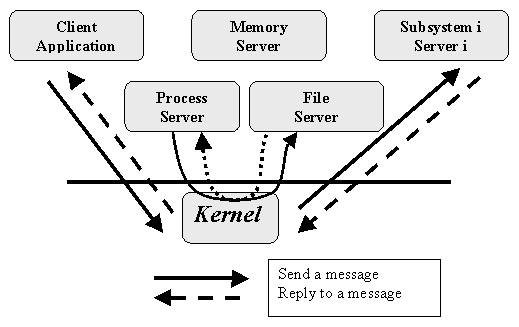
\includegraphics[width=0.8\linewidth]{figs/1kernel.png}
	\end{center}

 	   \column{.30\textwidth}
	\begin{block}{Advantages}
	\begin{itemize}
		\item Robustness
		\item Modularity
		\item Distributed
	\end{itemize}
	\end{block}

	\begin{block}{Disadvantages}
	\begin{itemize}
		\item Complexity
	\end{itemize}
	\end{block}
	\end{columns}
\end{frame}

\begin{frame}{Overview (II)}
    \begin{columns}
 	   \column{.40\textwidth}
		Key ROS concepts

 	 	\begin{itemize}
		\item Node: Like a process
		\item Topic: Like a message blackboard
		\end{itemize}

		Key ROS commands
 	 	\begin{itemize}
		\item \texttt{roscore}: Runs core nodes in ROS
		\item \texttt{rosrun}: Runs a node
		\item \texttt{roslaunch}: Runs several nodes
		\end{itemize}

 	   \column{.60\textwidth}
	   \begin{block}{Practice}
	   \small{
	   \texttt{> roscore}\\
	   \texttt{> rosrun turtlesim turtlesim\_node}\\
	   \texttt{> rosrun turtlesim turtle\_teleop\_key}\\
	   \texttt{> rosrun rqt\_graph rqt\_graph}\\
	   }
	   \end{block}
	   \bigskip
		\centering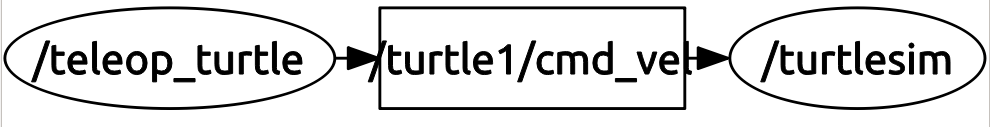
\includegraphics[width=\linewidth]{figs/captura2.png}\\
		\bigskip
		\centering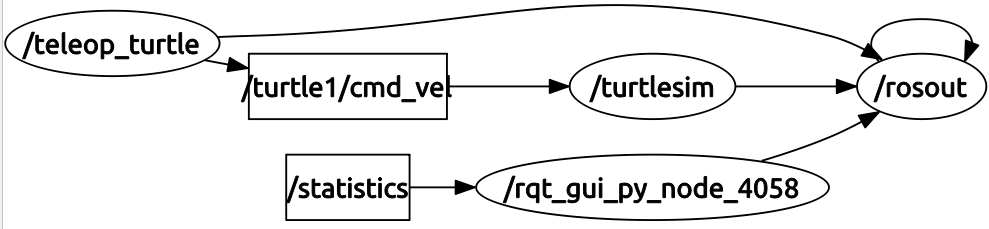
\includegraphics[width=\linewidth]{figs/captura1.png}
	\end{columns}
\end{frame}

\begin{frame}{Overview (III)}
	ROS defines a three-level architecture
	\begin{itemize}
		\item The community level
		\item The computation graph level
		\item The filesystem level
  	\end{itemize}
\end{frame}

\section{The community level}
\begin{frame}{The community level}
	Resources to distribute software and share knowledge
  	\begin{itemize}
		\item Distributions
		\item Repositories
		\item Wiki
		\item Forum
	\end{itemize}
\end{frame}

\section{The computation graph level}
\begin{frame}{The computation graph level}
	ROS creates a network of processes (nodes) communicated by different means
  	\begin{itemize}
		\item Nodes, Master, Parameter server, Messages, Topics, Services and Bags
	\end{itemize}
	\begin{center}
	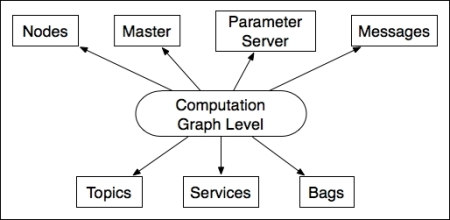
\includegraphics[width=0.5\linewidth]{figs/graph.jpg}
	\end{center}
\end{frame}

\subsection{Nodes}
\begin{frame}{The computation graph level}{Nodes (I)}
	\textbf{Node}: Information processing unit in ROS\\
	\begin{itemize}
	\item One node, one specific function
  	\begin{itemize}
		\item One node controls a motor, another one the ultrasound sensor, etc
	\end{itemize}
	\item Increased security and fault tolerance
	\item Unique name
	\item Nodes implemented in C++, Python or Matlab
	\end{itemize}
\end{frame}

\begin{frame}{The computation graph level}{Nodes (II)}
	A handy command-line utility: \alert{\texttt{rosnode}}
  	\begin{itemize}
		\item \texttt{rosnode list}
		\item \texttt{rosnode info node}
		\item \texttt{rosnode kill node}
	\end{itemize}
	Other utilities
  	\begin{itemize}
		\item \texttt{rosnode machine hostname}
		\item \texttt{rosnode ping node}
		\item \texttt{rosnode cleanup}
	\end{itemize}
\end{frame}

\begin{frame}{The computation graph level}{Nodes (III)}
	\begin{block}{Exercises}
  	\begin{itemize}
		\item Run the turtlebot simulation
			\begin{enumerate}
			\item \texttt{> rosrun turtlesim turtlesim\_node}
			\item \texttt{> rosrun turtlesim turtle\_teleop\_key}
			\end{enumerate}
		\item Identify the running nodes
		\item Get info about the node that runs the simulation
		\item Check connectivity with that node
		\item Kill the node
	\end{itemize}
	\end{block}
\end{frame}

\subsection{Topics}
\begin{frame}{The computation graph level}{Topics (I)}
	\textbf{Topic}: Communication buses used by nodes to transmit data
	\begin{itemize}
	\item Publisher/subscriber mechanism
	\item One-to-many communication
	\item Unique name
	\item Strongly typed
	\end{itemize}
	\begin{center}
	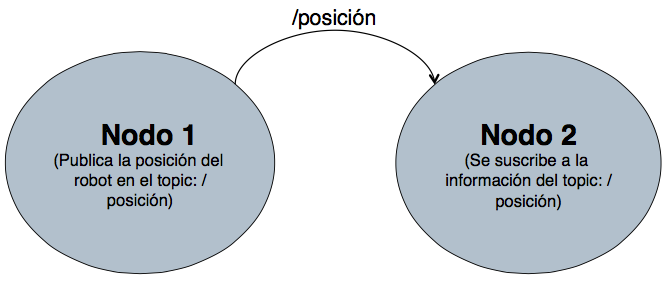
\includegraphics[width=0.4\linewidth]{figs/topic1.png}
	\end{center}
\end{frame}

\begin{frame}{The computation graph level}{Topics (II)}
	A handy command-line utility: \alert{\texttt{rostopic}}
  	\begin{itemize}
		\item \texttt{rostopic list}
		\item \texttt{rostopic echo topic}
		\item \texttt{rostopic info topic}
		\item \texttt{rostopic find message\_type}
	\end{itemize}
	Two pretty useful commands
  	\begin{itemize}
		\item \texttt{rostopic pub topic type args}
		\item \texttt{rostopic type topic}
	\end{itemize}
\end{frame}

\begin{frame}{The computation graph level}{Topics (III)}
	\begin{block}{Exercises}
  	\begin{itemize}
		\item Run the turtlebot simulation
			\begin{enumerate}
			\item \texttt{> rosrun turtlesim turtlesim\_node}
			\item \texttt{> rosrun turtlesim turtle\_teleop\_key}
			\end{enumerate}
		\item Identify the available topics
		\item Which topic publishes the turtle motion?
		\item Visualize that topic while you teloperate the turtle
	\end{itemize}
	\end{block}
\end{frame}


\subsection{Services}
\begin{frame}{The computation graph level}{Services (I)}
	\textbf{Service}: RPC-like communication
	\begin{itemize}
	\item Strongly typed
	\item One-to-one communication
	\end{itemize}
	\begin{center}
	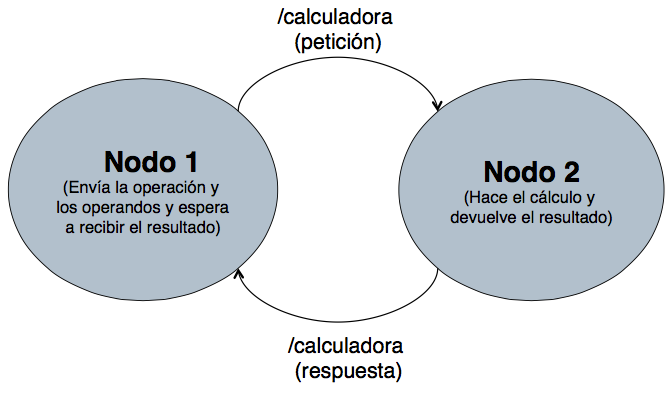
\includegraphics[width=0.45\linewidth]{figs/topic2.png}
	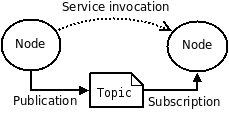
\includegraphics[width=0.45\linewidth]{figs/topic.png}
	\end{center}
\end{frame}

\begin{frame}{The computation graph level}{Services (II)}
	\vspace{-0.2cm}
	\begin{center}
	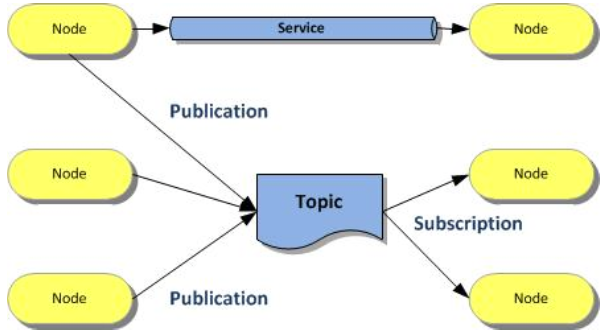
\includegraphics[width=0.6\linewidth]{figs/comparativa.png}
	\end{center}
	\vspace{-0.2cm}
	A handy command-line utility: \alert{\texttt{rosservice}}
  	\begin{itemize}
		\item \texttt{rosservice list}
		\item \texttt{rosservice info service}
		\item \texttt{rosservice call service}
		\item \texttt{rosservice type service}
	\end{itemize}
\end{frame}

\begin{frame}{The computation graph level}{Services (III)}
	\begin{block}{Exercises}
  	\begin{itemize}
		\item Run the turtlebot simulation
			\begin{enumerate}
			\item \texttt{> rosrun turtlesim turtlesim\_node}
			\item \texttt{> rosrun turtlesim turtle\_teleop\_key}
			\end{enumerate}
		\item Identify the available services
		\item Get information about the \texttt{spawn} service
		\item Find out the parameter type used by the service \texttt{reset}
		\item Call \texttt{spawn} with correct arguments
		\item Idenfity again the available services
	\end{itemize}
	\end{block}
\end{frame}

\subsection{Messages}
\begin{frame}[fragile]{The computation graph level}{Messages (I)}
	\textbf{Message}: Data structure used by nodes to communicate
  	\begin{itemize}
		\item \texttt{rosmsg list}
		\item \texttt{rosmsg show}
		\item \texttt{rosmsg package package}
		\item \texttt{rosmsg packages}
	\end{itemize}

    \begin{columns}
 	   \column{.50\textwidth}
	\begin{exampleblock}{Twist}
	\begin{verbatim}
Vector3  linear
Vector3  angular
\end{verbatim}
	\end{exampleblock}
 	   \column{.50\textwidth}
	\begin{exampleblock}{Vector3}
	\begin{verbatim}
float64 x
float64 y
float64 z
\end{verbatim}
	\end{exampleblock}
	\end{columns}
\end{frame}

\begin{frame}{The computation graph level}{Messages (II)}
	\begin{center}
	\large{Data types}
	\vspace{0.3cm}
	\begin{tabular}{lc} \hline
	{\sc Type} & {\sc Keyword} \\ \hline
	Integer & int8, int16, int32, int64 (plus uint*)\\ 
	Float & float32, float64\\ 
	String & string\\ 
	Time & time, duration\\ 
	Struct & other msg files\\ 
	Array &variable-length array[] and fixed-length array[C]\\ \hline
	\end{tabular}
	\end{center}
\end{frame}

\subsection{Others}
\begin{frame}{The computation graph level}{Others (I)}
	\begin{itemize}
	\item \textbf{Bags}: File contaning messages, topics, services and others. Usefull for debugging
	\item \textbf{Master}: Naming and registration services. Run by \texttt{roscore}. Provides the parameter server
	\item \textbf{Parameter server}: Dictionary that stores shared parameters, implemented with XML-RPC
  	\begin{itemize}
		\item \texttt{rosparam list}
		\item \texttt{rosparam get parameter}
		\item \texttt{rosparam set parameter parameter}
	\end{itemize}
	\end{itemize}
\end{frame}

\begin{frame}{The computation graph level}{Others (II)}
	\begin{block}{Exercises}
  	\begin{itemize}
		\item Run the turtlebot simulation
			\begin{enumerate}
			\item \texttt{> rosrun turtlesim turtlesim\_node}
			\item \texttt{> rosrun turtlesim turtle\_teleop\_key}
			\end{enumerate}
		\item Identify the available messages
		\item Extract the message format used to move the turtle
		\item Move the turtle using \texttt{rostopic}
		\item Identify the available parameters
		\item Get ROS version and distro name by using parameters
		\item Change the background color of the turtle simulation
	\end{itemize}
	\end{block}
\end{frame}

\begin{frame}{The computation graph level}{Practice}
	\begin{itemize}
		\item Run the Hector UAV simulation
		\begin{enumerate}
			\item \texttt{> roslaunch hector\_quadrotor\_demo outdoor\_flight\_gazebo.launch}
			\item \texttt{> roslaunch hector\_quadrotor\_teleop xbox\_controller.launch}
		\end{enumerate}
		\item Identify the node that publishes the UAV motion
		\item Move the UAV using \texttt{rostopic}
		\item Visualize in real-time the laser scan messages
		\item Explore and understand the laser scan message format
	\end{itemize}
\end{frame}

\section{The filesystem level}
\begin{frame}{The filesystem level}
    \begin{columns}
 	   \column{.60\textwidth}
	   \small{
		ROS resources stored on disk
  		\begin{itemize}
			\item \textbf{Packages}: Main unit of organization
			\item \textbf{Metapackages}:Collection of packages
			\item \textbf{Package Manifests}: Metadata about a package (\texttt{package.xml})
			\item \textbf{Repositories}: Collection of packages sharing a common VCS system
			\item \textbf{Message types}: Message descriptions
			\item \textbf{Service types}: Service descriptions
		\end{itemize}
		}
	   \column{.50\textwidth}
			\centering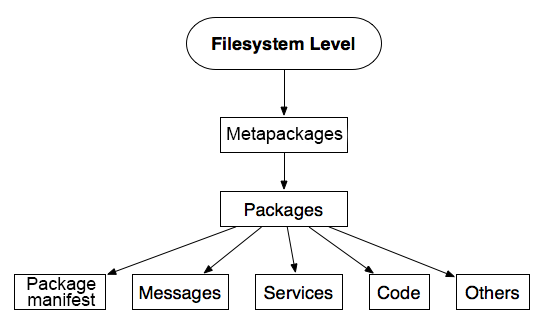
\includegraphics[width=\linewidth]{figs/filesystem.png}
	\end{columns}

\end{frame}

\subsection{Packages}
\begin{frame}{The filesystem level}{Packages (I)}
    \begin{columns}
 	   \column{.40\textwidth}
			\centering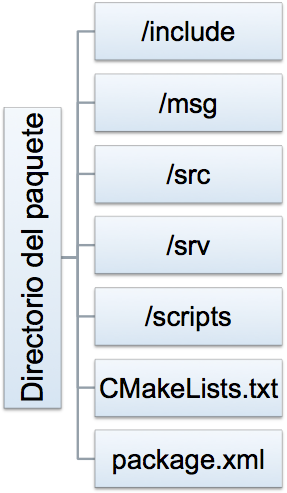
\includegraphics[width=0.9\linewidth]{figs/package.png}
	   \column{.60\textwidth}
	A package contains
  	\begin{itemize}
		\item One or more nodes
		\item Messages description
		\item Services description
		\item ROS libraries
		\item Config files
	\end{itemize}
	\begin{block}{Exercises}
	\begin{enumerate}
		\item Go to \texttt{/opt/ros/indigo/share/}
		\item List the ROS packages installed
		\item Browse the package \texttt{turtlesim}
	\end{enumerate}
	\end{block}
	\end{columns}
\end{frame}

\begin{frame}{The filesystem level}{Packages (II)}
	Several tools to manage ROS package
	\begin{itemize}
		\item \texttt{rospack list}
		\item \texttt{rospack find package}
	\end{itemize}
    \hspace{1cm}\begin{columns}
 	   \column{.40\textwidth}
	To move
	\begin{itemize}
		\item \texttt{roscd}
		\item \texttt{roscd package}
		\item Try \texttt{roscd log}
	\end{itemize}
 	   \column{.40\textwidth}
	To list
	\begin{itemize}
		\item \texttt{rosls}
		\item \texttt{rosls package}
	\end{itemize}
	\end{columns}
	\bigskip
	Package path \textit{must} be contained in \texttt{\$ROS\_PACKAGE\_PATH}\\
	Hint: Tab completion
\end{frame}

\subsection{Important ROS packages}
\begin{frame}{The filesystem level}{Important ROS packages}
\begin{center}
  \begin{tabular}{cl} \hline
  	{\sc Package} 		& {\sc Description} \\ \hline 
	\texttt{roscpp} 	& C++ client library     \\ 
	\texttt{rospy} 		& Python client library     \\ \hline
	\texttt{std\_msgs}	& Standard messages     \\ 
	\texttt{geometry\_msgs}	& Geometric messages     \\ \hline
	\texttt{TF} 		& Coordinate systems mapping     \\ 
	\texttt{gmapping} 	& SLAM based on laser sensors     \\ 
	\texttt{amcl} 		& 2D Monte Carlo localization     \\ \hline
	\texttt{stdr\_simulator} & STDR simulator   \\ 
	\texttt{stage\_ros}	& Stage simulator   \\ 
	\texttt{gazebo\_ros\_pkgs} & Interface for Gazebo   \\ \hline
    \end{tabular}
\end{center}

\end{frame}

\subsection{Messages types}
\begin{frame}[fragile]{The filesystem level}{Messages types (I)}
	Messages types define data structures 
  	\begin{itemize}
		\item Stored in a \texttt{.msg} file
		\item Folder \texttt{/msg}
		\item Automatic code generation
		\item Well documented in the Web
	\end{itemize}
	\begin{exampleblock}{\texttt{geometry\_msgs/Twist.msg}}
	\begin{verbatim}
# This expresses velocity in free space broken
# into its linear and angular parts.
Vector3  linear
Vector3  angular
\end{verbatim}
	\end{exampleblock}
\end{frame}

\begin{frame}[fragile]{The filesystem level}{Messages types (II)}
	\begin{exampleblock}{\texttt{geometry\_msgs/Vector3.msg}}
	\begin{verbatim}
float64 x
float64 y
float64 z
\end{verbatim}
	\end{exampleblock}

	\begin{block}{Exercise}
	\begin{enumerate}
		\item Move to the \texttt{turtlesim} package folder
		\item Identify the messages defined by the package \texttt{turtlesim}
		\item Visualize the message file \texttt{Color.msg}
	\end{enumerate}
	\end{block}
\end{frame}

\subsection{Service types}
\begin{frame}[fragile]{The filesystem level}{Service types (I)}
	Service types define the request and response structure
  	\begin{itemize}
		\item Stored in a \texttt{.srv} file
		\item Folder \texttt{/srv}
		\item Automatic code generation
		\item Well documented in the Web
	\end{itemize}

	\begin{exampleblock}{\texttt{turtlesim/srv/Spawn.srv}}
	\begin{verbatim}
float32 x
float32 y
float32 theta
string name # Optional.  A unique name will be
            # created and returned if this is empty
---
\end{verbatim}
	\end{exampleblock}
\end{frame}

\begin{frame}[fragile]{The filesystem level}{Service types (II)}
	\begin{block}{Exercise}
	\begin{enumerate}
		\item Move to the \texttt{turtlesim} package folder
		\item Identify the services defined in the package
		\item Visualize their format
	\end{enumerate}
	\end{block}
\end{frame}

\subsection{Others}
\begin{frame}{The filesystem level}{Others}
	\textbf{Package Manifests}: Metadata about a package
  	\begin{itemize}
		\item Package name, version, dependences, etc
		\item Stored in the \texttt{package.xml} file
		\item XML format
	\end{itemize}
	\textbf{Metapackages}: Package that contains other packages
  	\begin{itemize}
		\item It only installs one file: \texttt{package.xml}
		\item Uses to contain specialized features
	\end{itemize}
	\textbf{Repositories}: Collection of packages sharing a VCS system
	\begin{block}{Exercises}
	\begin{enumerate}
		\item Go to the \texttt{turtlesim} package root folder
		\item Read its package manifiest file
		\item Which dependences does \texttt{turtlesim} have?
	\end{enumerate}
	\end{block}
\end{frame}

%\section{Exercises}
%\begin{frame}{Exercises}
%	TODO
%\end{frame}

\section{Node execution}
\subsection{Single node (\texttt{rosrun})}
\begin{frame}{Node execution}{Single node (\texttt{rosrun})}
	\textbf{rosnode}: Executes a single node
    \begin{columns}
 	   \column{.80\textwidth}
	   \begin{block}{}
	   \texttt{rosrun <package> <node> [parameters]}
	   \end{block}
	\end{columns}
	\bigskip
	Example: \texttt{rosrun my\_package my\_node \_my\_param:=value}\\
	\bigskip
	Warning: The node must be in \texttt{\$ROS\_PACKAGE\_PATH}! (ROS init scripts)
\end{frame}

\subsection{Several nodes (\texttt{roslaunch})}
\begin{frame}{Node execution}{Several nodes (\texttt{roslaunch}) (I)}
	Usually, any ROS application is composed of several nodes
	\begin{itemize}
		\item Executing each node is unefficient
		\item Automate node execution
	\end{itemize}

	Features
	\begin{itemize}
		\item Run one or several nodes, group nodes, set up parameters, define environment variables, remap topics, respawn nodes
	\end{itemize}

	\href{http://wiki.ros.org/roslaunch}{(More info)}\\
	\textbf{roslaunch}: Node execution control
    \begin{columns}
 	   \column{.80\textwidth}
	   \begin{block}{}
	   \texttt{roslaunch <package\_name> <file.launch>}
	   \end{block}
	\end{columns}
	\bigskip

\end{frame}

\begin{frame}{Node execution}{Several nodes (\texttt{roslaunch}) (II)}
	\vspace{-0.2cm}
	roslaunch uses an XML file
	\begin{itemize}
	\item Usually stored in the \texttt{launch} folder
	\end{itemize}

	\vspace{-0.2cm}
    \begin{exampleblock}{launch/minimal.launch (rospy\_tutorials package)}
		\vspace{-0.2cm}
	    \lstinputlisting[language=xml, basicstyle=\ttfamily\scriptsize]{code/minimal.xml}
		\vspace{-0.2cm}
    \end{exampleblock}

	Launch files might be quite complex

	\vspace{-0.2cm}
    \begin{exampleblock}{launch/server\_no\_map.launch (stdr\_launchers package)}
		\vspace{-0.2cm}
	    \lstinputlisting[language=xml, basicstyle=\ttfamily\scriptsize]{code/servernomap.launch}
		\vspace{-0.2cm}
    \end{exampleblock}

\end{frame}


\begin{frame}[fragile,plain]{Node execution}{Several nodes (\texttt{roslaunch}) (III)}
	\vspace{-0.2cm}
    \begin{exampleblock}{Minimal launch file}
		\vspace{-0.2cm}
	    \lstinputlisting[language=xml, basicstyle=\ttfamily\tiny]{code/complex.xml}
		\vspace{-0.2cm}
    \end{exampleblock}
\end{frame}

\begin{frame}{Node execution}{Several nodes (\texttt{roslaunch}) (IV)}
	\begin{block}{Exercise}
	\begin{enumerate}
		\item Move to the \texttt{stdr\_launchers} package folder
		\item Follow this tutorial: \url{http://wiki.ros.org/stdr\_simulator/Tutorials/Running\%20STDR\%20Simulator}
		\item For each execution of \texttt{roslaunch}, open and read the launch file
	\end{enumerate}
	\end{block}
\end{frame}


\end{document}
